\newpage{\ } 
\thispagestyle{empty} 

\chapter{Retinopatía diabética}
\lhead{Capítulo 2. \emph{Retinopatía diabética}} % This is for the header on each page - perhaps a shortened title


Desde el punto de vista oftalmológico, la retinopatía diabética es un problema de salud pública de gran magnitud ya que es una de las causas principales de ceguera a nivel mundial \cite{nei}. Esta enfermedad ocurre cuando la diabetes daña a los pequeños vasos sanguíneos de la retina, que es el tejido sensible a la luz situado en la parte posterior del ojo. En la FIGURA  \ref{fig:retino_eye} se puede apreciar con más detalle la estructura del ojo y sus partes.
La ceguera o pérdida de la visión se puede prevenir mediante la detección temprana y un tratamiento adecuado. La detección temprana de la retinopatía diabética es rentable respecto al costo económico  del tratamiento en personas con diabetes \cite{fong9394vision}. %Existe un consenso generalizado de que la detección temprana regular de la retinopatía diabética, se requiere y es rentable en las personas con diabetes \cite{fong9394vision}.  

La obtención y lectura experta de imágenes de retina  ha demostrado ser comparable o superior a una visita al consultorio para evaluar la presencia de retinopatía diabética en los ojos \cite{lin2002sensitivity}. Esta obtención y lectura se ha propuesto como un método para hacer el examen de ojo dilatado a poblaciones desatendidas que no reciben exámenes regulares de los proveedores de atención oftálmica. 

La mayoría de los programas de detección temprana o programas de detección utilizan cámaras de fondo de color digital para adquirir fotografías en color de la parte posterior del ojo, la retina \cite{jose2003camara}. Estas fotografías son examinadas por los expertos humanos para verificar la presencia de lesiones específicas que son indicativos de la retinopatía diabética.


    \begin{figure}[!hbtp]
	\centering
		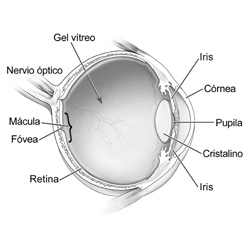
\includegraphics[width=0.5	\textwidth]{./Figures/retino_eye.jpg}
	\caption{Estructura del ojo.}
	\label{fig:retino_eye}
\end{figure}

\section{Diabetes}
%La Diabetes es % un grupo de enfermedades metabólicas caracterizadas por hiperglicemia, consecuencia de defectos en la secreción de la insulina, en la acción de la insulina ó en ambas. La hiperglicemia crónica se asocia a largo plazo a daños, disfunciónes e insuficiencia de diferentes órganos especialmente de los ojos, riñones, nervios, corazón y vasos sanguíneos  \cite{american2008diagnosis}. 

La Diabetes es una enfermedad crónica que requiere cuidado médico continuo y cuidado por parte del paciente para prevenir complicaciones agudas y reducir las mismas a largo plazo \cite{wagner2001improving}.

%Varios procesos patogénicos están involucrados en el desarrollo de la DM, desde la destrucción autoinmune de las células ß del páncreas con la consecuente deficiencia de insulina hasta las anomalías que provocan resistencia a la acción de la insulina.
Las complicaciones a largo plazo de la diabetes incluyen la retinopatía con pérdida potencial de visión; la nefropatía que puede conducir a un fallo renal; la neuropatía periférica con el riesgo de ulceraciones, amputaciones y articulaciones; y la neuropatía autonómica que puede ocasionar trastornos gástricos, genitourinarios cardiovasculares, así como disfunción sexual.
La gran mayoría de los casos de diabetes se dividen en dos grandes categorías: diabetes de tipo I (DI) y de tipo II (DII). En la primera de ellas, la causa es una deficiencia absoluta en la secreción de insulina, a menudo con evidencia de destrucción
autoinmune de las células $\beta$ pancreáticas. 
\nomenclature[]{$\beta$}{Células Beta.}%
En la segunda categoría, la más común, la causa es una combinación de resistencia a la acción de la insulina (generalmente asociada a la obesidad) y una inadecuada respuesta secretora compensatoria \cite{alfaro2000tratamiento}.
\section{Tipos de Diabetes}
Se sabe que la mayoría de las personas que desarrollan diabetes no lo hacen de forma repentina. Se trata de un proceso que puede durar años, incluso iniciarse desde el nacimiento. En este contexto, se menciona  los tipos de diabetes \cite{ceocomplicaciones}.
\subsection{Tipo I}
Se caracteriza por el déficit total de insulina debido a la destrucción de las células del páncreas. En
la mayoría de los casos tiene una base autoinmune, con factores genéticos implicados, aunque el mecanismo desencadenante de la respuesta inmune aún no está clarificado. Afecta fundamentalmente a personas jóvenes, que deberán mantener un tratamiento dietético con administración de insulina de por vida. Supone aproximadamente el 10\% de los distintos
tipos de diabetes \cite{mellitus2004diabetes}

\subsection{Tipo II}
Llamada anteriormente ``diabetes del adulto", es el tipo más común y los individuos tienen un déficit relativo de insulina. En este tipo predomina la resistencia a la insulina sobre el defecto de la secreción,
aunque habitualmente coexisten ambos problemas. No hay destrucción de células y la secreción de insulina es variable, a veces superior a lo normal, pero insuficiente para vencer el grado de insulinorresistencia.
En su etiología subyace una predisposición genética, pero los factores ambientales ejercen un importante
papel en su aparición, entre ellos, una alimentación inadecuada, el sedentarismo y la obesidad \cite{mellitus2004diabetes}.

\subsection{Diabetes en Paraguay}
En marzo de 2014 el Programa Nacional de Diabetes estimó que existen unas 700.000 personas (11\% de la población) en riesgo de desarrollar la afección y 400.000 en tratamiento \cite{20medios}. 
\subsection{Aumento de la prevalencia de la diabetes}
La cantidad de personas con diabetes ha ido en aumento, esperándose que de las 171 millones de personas con esta enfermedad desde el año 2000, aumente a 336 millones para el 2030, con un incremento de un 86\%. En Latinoamérica aumentará de 13,3 millones a 33 millones para el año 2030 con incremento de 146\% \cite{wild2004global}. Una estimación del aumento de los casos de diabetes hacia el año 2030, realizada por la Federación Internacional de Diabetes \cite{idf} se muestra en la TABLA \ref{tab:futuro}.


\begin{table}[!hbtp]
\begin{center}
\small

\caption{Estimación del aumento de los casos de Diabetes al año 2030 para países de Latinoamérica, de acuerdo a la Federación Internacional de Diabetes.}
\label{tab:futuro}
\begin{tabular}{|c|c|c|c| p{2cm}}
\hline
País &  Año 2000 & Año 2030 & Aumento de los casos
 \\ 
\hline
Argentina & 1.426.000 & 2.457.000 & 72,30\% \\
Baharmas & 12.000 &26.000 & 116,6\%\\
Bolivia & 207.000& 562.000 & 171,49\%\\
Brasil & 4.553.000 & 11.305.000 & 148, 29\%  \\
Chile & 495.000 & 1.047.000 & 111,51\%  \\
Colombia & 883.000 & 2.425.000 & 174,63\%   \\
Costa Rica & 76.000& 237.000 & 211,84\%\\
Cuba&480.000& 855.000 & 178,12\%\\
República Dominicana& 245.000& 594.000 & 142,4\% \\
Ecuador & 341.000 & 921.000 & 170\%  \\
El Salvador&103.000&320.000 & 210,6\%\\
Guatemala& 139.000& 447.000 & 221,58\%\\
Haití&  161.000& 401.000 & 149\%\\
Honduras&81.000& 269.000 & 232\%\\
Jamaica& 81.000&189.000 & 133,33\%\\
México&2.179.000& 6.130.000 & 181,32\%\\
Nicaragua&68.000&246.000 & 261,76\%\\
Panama&59.000&155.000 & 162,71\%\\
\textbf{Paraguay} & \textbf{102.000} & \textbf{324.000} & \textbf{217,64}\%  \\
Perú & 754.000 & 1.961.000 & 160,07 \% \\
Trinidad y Tobago&60.000&125.000 & 108,3\%\\
Uruguay& 154.000& 224.000 & 45,45\%\\


\hline
\end{tabular}


\end{center}

\end{table}

\section{Enfermedades del Ojo}
La enfermedad diabética del ojo se refiere a un grupo de problemas de los ojos que pueden desarrollarse en las personas con diabetes. Todos estos problemas pueden causar una pérdida de visión severa o incluso la ceguera.
La enfermedad diabética del ojo puede incluir:
\begin{itemize}
\item Retinopatía diabética: daño en los vasos sanguíneos de la retina.

\item Cataratas: se produce cuando el cristalino (el ``lente" del ojo) se nubla.

\item Glaucoma: ocurre cuando el líquido dentro del ojo drena muy lentamente. Cuando se acumula este líquido, la presión dentro del ojo aumenta y puede dañar el nervio óptico y causar la pérdida de su visión.
\end{itemize}
\section{Reseña sobre retinopatía diabética}
Se entiende por retinopatía diabética como una complicación de los ojos provocada por la diabetes que está causada por el deterioro de los vasos sanguíneos, glaucoma y cataratas. Como consecuencia del avance de la enfermedad la visión se deteriora debido a que la imagen enviada al cerebro se hace borrosa. 

\subsection{Causas}



Cuando los niveles de azúcar en la sangre son muy altos durante largos períodos de tiempo, los capilares (pequeños vasos sanguíneos) que suministran sangre a la retina pueden deteriorarse. Con el tiempo, estos vasos sanguíneos comienzan a filtrar líquidos y grasas, produciendo un edema (hinchazón). Eventualmente, puede ocurrir una condición llamada isquemia, durante el cual los vasos sanguíneos pueden taparse. Estos problemas son asociados a la presencia de la retinopatía diabética \cite{AAOcausas}.

\subsection{Factores de riesgo}

El tiempo de duración de la diabetes es el principal factor de riesgo, después de 15 años de diabetes, el 97,5\% de los pacientes con diabetes tipo I y el 77,8\% de los pacientes con diabetes tipo II, padecen algún grado de retinopatía diabética. En este sentido, el control metabólico es de crucial importancia para prevenir la aparición o disminuir la progresión de la retinopatía diabética. Según el ensayo sobre el control y complicaciones de la diabetes, el control intensivo de la glucemia reduce el riesgo de desarrollar retinopatía diabética en un 76\%, y retarda su progresión en un 54\%. Otros factores como la hipertensión arterial están asociadas a mayor riesgo de progresión del edema macular y de la retinopatía diabética en general, cuando no está controlada en forma crónica. %La nefropatía por su parte tiene un efecto adverso en la retinopatía diabética. 
Los diabéticos tipo I con micro albuminuria tienen tres veces más probabilidades de tener retinopatía diabética. El embarazo acelera la progresión de la retinopatía diabética, por lo que las mujeres diabéticas embarazadas requieren controles de retina más frecuentes \cite{retinoUSdep,AAORiesgos}.

%Las personas con diabetes están en riesgo de desarrollar retinopatía diabética. 
%La diabetes es una enfermedad que afecta la capacidad del cuerpo para producir o utilizar insulina de manera eficaz para controlar los niveles de azúcar en la sangre \cite{AAORiesgos}.



\subsection{Síntomas}

A medida que la enfermedad progresa, los síntomas de la retinopatía diabética pueden incluir \cite{AAOSintomas}:
\begin{itemize}
\item Manchas, puntos o algo similar a hilos de telarañas oscuras flotando en la visión (llamados miodesopsias, manchas flotantes o “moscas” volantes);
\item Visión borrosa;
\item Visión que cambia periódicamente de borrosa a clara;
\item Áreas oscuras (completa o parcialmente) en el campo de visión;
\item Mala visión nocturna;
\item Colores que aparecen descoloridos o diferentes;
\item Pérdida de la visión.
Los síntomas de la retinopatía diabética afectan, por lo general, a ambos ojos. 

\end{itemize}



\subsection{Etapas de la retinopatía diabética}
La retinopatía diabética tiene cuatro fases \cite{diabetica2006pontificia}:

\textbf{Retinopatía no proliferativa leve:} en esta fase inicial se producen microaneurismas, que son pequeñas áreas de inflamación en forma de globo en los diminutos vasos sanguíneos de la retina.

\textbf{Retinopatía no proliferativa moderada:} a medida que la enfermedad avanza, se produce el bloqueo de algunos de los vasos sanguíneos que alimentan la retina.

\textbf{Retinopatía no proliferativa grave:} se produce el bloqueo de muchos más vasos sanguíneos, lo cual impide el aporte sanguíneo a diversas áreas de la retina. Estas áreas de la retina envían señales al cuerpo para que cree nuevos vasos sanguíneos para poder alimentarse.

\textbf{Retinopatía proliferativa:} en esta fase avanzada, las señales enviadas por la retina para su alimentación desencadenan el crecimiento de nuevos vasos sanguíneos. Estos nuevos vasos sanguíneos son anormales y frágiles. Crecen a lo largo de la retina y de la superficie del gel vítreo transparente que llena el interior del ojo. Por sí solos, estos vasos sanguíneos no causan síntomas ni pérdida de visión. Sin embargo, sus paredes son delgadas y frágiles. Si presentan filtraciones de sangre, puede producirse una pérdida grave de visión e incluso la ceguera \cite{optos}.


\subsection{Tratamiento}
Durante las tres primeras etapas de la retinopatía diabética no se necesita un tratamiento, a menos que tenga edema macular. Para prevenir el progreso de la retinopatía diabética, las personas con diabetes deben controlar los niveles de azúcar en la sangre, la presión arterial y el colesterol \cite{retinoUSdep}.

%La retinopatía proliferativa se trata con cirugía láser. Este procedimiento se llama fotocoagulación retiniana. Este tratamiento ayuda a reducir los vasos sanguíneos anormales. Su oculista le 
%hará entre mil y dos mil quemaduras con láser en las áreas de la retina lejos de la mácula, haciendo que se achiquen los vasos sanguíneos anormales. Debido a que es necesario realizar muchas quemaduras con láser, usualmente se necesitan dos sesiones o más para completar el tratamiento. Aunque usted puede notar que ha perdido alguna de su visión lateral, la fotocoagulación retiniana puede preservarle el resto de su visión. Este tratamiento puede reducirle un poco su visión de color y su visión de noche \cite{retinoUSdep}. 

%El tratamiento de fotocoagulación retiniana funciona mejor antes de que los nuevos y frágiles vasos sanguíneos empiecen a sangrar. 
%Por eso es muy importante hacerse regularmente un examen completo de la vista con dilatación de las pupilas. Aún cuando usted ya haya empezado a sangrar, es posible que todavía se pueda hacer el tratamiento de fotocoagulación retiniana, dependiendo en la cantidad de la hemorragia.
%Si la hemorragia es severa, usted puede necesitar un procedimiento quirúrgico llamado vitrectomía (vea a continuación). Durante una vitrectomía, se quita la sangre del centro de su ojo \cite{retinoUSdep}.

%Es difícil hacer el suficiente hincapié en que el tratamiento comienza por lograr que el paciente tome conciencia de su enfermedad, de sus riesgos potenciales, y que acuda a controles periódicos con su diabetólogo y con su oftalmólogo \cite{diabetica2006pontificia}.

\subsubsection{Fotocoagulación  con Láser}
La fotocoagulación es un proceso no quirúrgico que consiste en realizar aplicaciones de láser térmico sobre la superficie retinal. Estas quemaduras destruyen la retina en el lugar en que son aplicadas, creando una cicatriz. 
%La racionalidad de este tratamiento se basa en que, al destruir la retina isquémica, ésta sería incapaz de producir el Factor de Crecimiento Vascular Endotelial, el que sería el responsable de la formación de los neovasos. La disminución de la producción de este factor soluble lograría la regresión de la neovascularización  existente y la prevención de su desarrollo en el futuro \cite{diabetica2006pontificia}.

 Antes de la existencia de la fotocoagulación, la retinopatía diabética conducía con frecuencia a la pérdida total de visión \cite{kanski2004oftalmologia}.
 
 \subsubsection{Terapia médica intravítrea}
 Los medicamentos intravítreos tienen un efecto temporal, por lo cual no sustituyen al tratamiento con láser. Dentro de estos se encuentran los esteroides (Triamcinolona o dexametasona de acción prolongada), usados en el edema macular, pero aumentan el riesgo de hipertensión ocular y de catarata, y los antiangiogénicos que mejoran el edema macular y reducen la neovascularización de la retina \cite{barria2011guia}.
 \subsubsection{Tratamiento quirúrgico}
 El tratamiento quirúrgico de la retinopatía diabética sólo es necesario en casos muy avanzados, fundamentalmente cuando se produce una hemorragia vítrea. La intervención se denomina vitrectomía y consiste en \cite{manteca2012tratamiento}:
 \begin{itemize}
 \item Aspirar la sangre de la hemorragia. 
 \item Fijar el desprendimiento de la retina.
  \item Completar el proceso con una fotocoagulación en la misma operación para evitar que se vuelva a repetir.
 \end{itemize}
 
 



\section{Detección de retinopatía diabética}

Para entender mejor la detección de retinopatía diabética es necesario definir que es un diagnóstico. Básicamente consiste en determinar la presencia o ausencia de una enfermedad, para este caso particular es la  presencia ó ausencia de la retinopatía diabética. Un diagnóstico positivo determina la presencia de retinopatía diabética y un diagnóstico negativo determina la ausencia de retinopatía diabética.
Cuando se habla de diagnóstico masivo se introduce el concepto de \textit{screening}, que no es más que la evaluación  de sujetos asintomáticos respecto a una patología específica, antes de que ellos consulten espontáneamente. Desde el punto de vista teórico, esta acción médica se justifica, cuando la enfermedad repercute en la vida de quienes la padecen, tenga una prevalencia importante, presente un tratamiento efectivo y cuente con un método de diagnóstico eficiente de alta sensibilidad \cite{uk2003criteria,beaglehole1994epidemiologia}.

El tamizaje ofrece una prueba a una población, en este caso a todos los pacientes con diabetes y aquellos positivos son referidos para mayor investigación o tratamiento. 
%Tamizaje deriva de la palabra tamiz, colador, filtro, o “\textit{screening}” en inglés, y como todo colador, a veces deja pasar casos que sí tienen la enfermedad y que no fueron detectados (falsos negativos), o puede identificar casos creyendo que sí tienen la enfermedad pero que en realidad no la presentan (falsos positivos). Los falsos negativos y los falsos positivos son inherentes a cualquier programa de tamizaje, sin embargo todo programa de este tipo debe minimizar el número de estos mediante un proceso de control de la calidad. Por lo tanto, tamizar es “reducir el riesgo” para una población específica, no eliminarlo por completo. 
El mayor cuidado que se debe tener en un programa de \textit{screening}, es tratar de disminuir los falsos negativos, estos son casos de personas con la enfermedad que fueron diagnosticadas como sanas \cite{von2011guia}.

La Organización Mundial de la Salud \cite{oms} estableció los 10 principios para establecer un programa de \textit{screening} de cualquier enfermedad \cite{zavon1969principles,wilson1968principles}: 
\begin{itemize}
\item La condición buscada debe ser un problema de salud importante. 
\item Debe existir  un tratamiento adecuado para los pacientes con la enfermedad detectada.
\item  Deben estar disponibles  las instalaciones para el diagnóstico y tratamiento. 
\item  Debe haber una etapa latente o sintomática temprana reconocible. 
\item  Debe haber una prueba o un examen adecuado.
\item  La prueba debe ser aceptable para la población. 
\item  La historia natural de la enfermedad, incluyendo el desarrollo latente de  la enfermedad, debe entenderse adecuadamente. 
\item  Debe haber una política de acuerdo sobre a quiénes tratar como pacientes. 
\item  El costo de la detección de casos (incluyendo el diagnóstico y el tratamiento de los pacientes diagnosticados) debe ser económicamente equilibrada en relación con posibles gastos en atención médica en su conjunto. 
\item La detección de casos debe ser un proceso continuo. 
\end{itemize}
Un programa de \textit{screening} de la retinopatía diabética
con cámara fotográfica digital se ajusta perfectamente a estos principios \cite{vision2020la} ya que la ceguera por retinopatía diabética es un problema de salud pública. Se conoce claramente su historia natural y su epidemiología, posee un periodo de latencia de varios años, se cuenta con un tratamiento adecuado como es el láser, se sabe a quién tratar, el costo de tratar a una persona en riesgo es mucho menor que el costo que genera un tratamiento en estados avanzados. %Contamos con los equipos para el diagnóstico y el tratamiento, poseemos una prueba sencilla, rápida, precisa e indolora como es la cámara fotográfica, y esta prueba es aceptada fácilmente por la población en riesgo. El último principio es que el tamizaje sea un proceso continuo y sistemático depende del proceso gerencial que realicemos, siendo este punto fundamental.

La retinopatía diabética es evitable con medidas preventivas, de ahí que el \textit{screening} sistemático de los diabéticos es de suma importancia. Esta metodología epidemiológica, consiste en la evaluación de individuos asintomáticos para detectar la enfermedad temprana.
La oftalmoscopia o estudio del fondo de ojo es una técnica de diagnóstico que consiste en visualizar el polo posterior del globo ocular, que incluye retina, disco óptico, coroides y vasos sanguíneos \cite{exa}. Existen varias manera de relizar un estudio de fondo de ojo. 
\begin{itemize}
\item Oftalmoscopia directa: técnica sencilla en la cual la exploración ocular se realiza mediante el uso de un oftalmoscopio monocular.
\item Oftalmoscopia indirecta: técnica en la cual la exploración ocular se realiza mediante el uso de un oftalmoscopio binocular y de una fuente de luz externa.
\item Biomicroscopia: o también conocida como oftalmoscopia indirecta con lámpara de hendidura técnica compleja en la cual la exploración ocular se realiza mediante el empleo de una lámpara de hendidura.
\item Cámara digital: a diferencia del oftalmoscopio, los retinógrafos o cámaras digitales  permiten obtener fotografías de la retina.
\end{itemize}

En la TABLA \ref{tab:screening} se observan las diferencias entre los métodos de estudio del fondo de ojo, donde dilatación se refiere a agrandar las pupilas, para permitir al oftalmólogo observar detalladamente el interior del ojo.

\begin{table}[!hbtp]
\begin{center}
\caption{Estudio del fondo de ojo. }
\resizebox{15cm}{!} {
\begin{tabular}{|c|c|c|c| c|c|c| p{2cm}}
\hline
 &Costo& Manejo & Disponibilidad& Sensitividad & Dilatación& Archivo\\ 
\hline
Oft. directo &Bajo&Facil&Si &Baja&Si&No\\
Oft. indirecto &Medio&Especial&No siempre&Buena&Si&No\\
Biomicroscopia & Medio & Especial & Casi Siempre & Optima Gold Standard & Si & No\\

Cámara digital & Ato &Fácil & A veces& Muy Buena & Si &Si   \\

\hline
\end{tabular}
}
\label{tab:screening}
\end{center}

\end{table}







Cualquier persona con diabetes debería someterse a una exploración ocular completa al menos una vez al año. Si tiene retinopatía diabética, puede que deba someterse a una exploración ocular más a menudo. Las personas con retinopatía proliferativa pueden reducir el riesgo de sufrir ceguera en un 95\% si reciben tratamiento a tiempo y se someten a un seguimiento adecuado. %Un importante estudio ha demostrado que un mejor control de los niveles de glucemia ralentiza la aparición y progresión de la retinopatía. Las personas con diabetes que mantuvieron sus niveles de azúcar en sangre lo más próximos posible a la normalidad también sufrieron muchas menos enfermedades renales y nerviosas. Un mejor control también reduce la necesidad de cirugía láser para conservar la vista. Este control del nivel de glucemia puede que no sea la mejor opción para todo el mundo, como los pacientes de edad más avanzada, los niños de menos de 13 años o las personas con cardiopatías. Consulte a su médico si un programa de control de este tipo es adecuado para usted. En otros estudios se ha demostrado que controlar la presión arterial y el colesterol elevados puede reducir el riesgo de pérdida de visión. El control de estos factores será beneficioso para su salud general, además de ayudar a proteger su vista.

La FIGURA \ref{fig:sinvscon1} muestra la comparación de la percepción visual entre  una persona con una retina sana y otra que sufre de retinopatía diabética, ya en una etapa avanzada de la enfermedad.
\begin{figure}[H]
\centering
\subfigure[Visión de una persona  sana.]{
\includegraphics[width=70mm, height=70mm]{./Figures/cap2/sinDR.png}}
\subfigure[Visión de una persona con retinopatía diabética en etapa avanzada.]{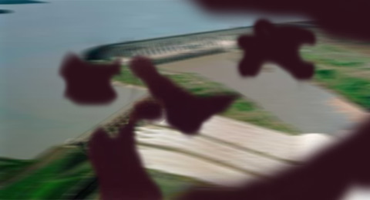
\includegraphics[width=70mm, height=70mm]{./Figures/cap2/conRD.png}}
\caption{Daño causado por la retinopatía diabética.} 
\label{fig:sinvscon1}
\end{figure}
\section{Estructuras anatómicas y patologías}
A continuación se expone en mayor detalle las estructuras anatómicas y patologías relacionadas con la retinopatía diabética, las cuales fueron consideradas en la etapa de detección del método propuesto.

\subsection{Microaneurismas}

Los microaneurismas son dilataciones que afectan a capilares de diversas áreas vasculares como el corazón, el riñón y el ojo. Los oftalmólogos saben que, si bien se presentan en varios procesos patológicos como hipertensión, oclusión venosa y alteraciones hemorreológicas, son característicos de la retinopatía diabética. En la FIGURA \ref{fig:sinvscon} se puede ver los microaneurismas en una imagen de retina.

\begin{figure}[H]
\centering
\subfigure[Imagen de Retina.]{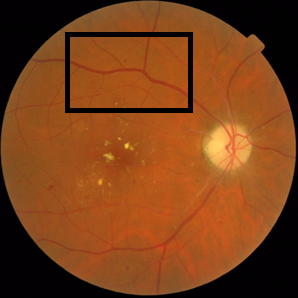
\includegraphics[width=70mm]{./Figures/cap2/microMu.png}}
\subfigure[Microaneurisma.]{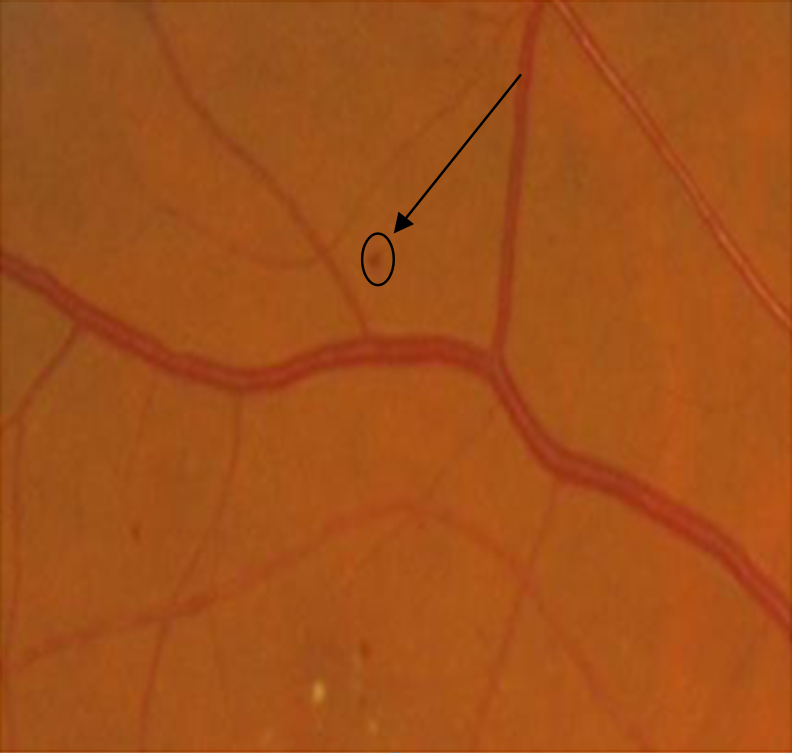
\includegraphics[width=70mm, height=70mm]{./Figures/cap2/microMu2.png}}
\caption{Microaneurismas.} \label{fig:sinvscon}
\end{figure}
\subsection{Exudados duros}
Los exudados duros son lípidos o depósitos lipoproteínicos usualmente localizados en la capa externa de la retina, ellos tienen una apariencia serosa como manchas blanquecinas de bordes bien definidos y son el resultado del escape de fluidos sanguíneos de los microaneurismas que son permeables, y también de los capilares pequeños que circundan la zona macular y que normalmente son impermeables. En algunas ocasiones tienen una forma de anillo redondeado que se denomina retinopatía circinada y son frecuentemente asociados con edema retinal. Elevados niveles de colesterol se correlacionan con más severas y extensas áreas de exudados duros. Sin embargo, un incremento en la severidad de los exudados duros no es asociado a un aumento de riesgo de progresión de la retinopatía. Bajos niveles de lípidos en sangre pueden ayudar a reducir la severidad de los exudados duros en la retina \cite{PedroSaenzRetinopatiaDiabetica}. En la FIGURA \ref{fig:sanosvsexu} se observa la diferencia entre una retina sana y una retina con exudados duros, los cuales se presentan como manchas amarillas con formas irregulares.

\begin{figure}[H]
\centering
\subfigure[Imagen de Retina.]{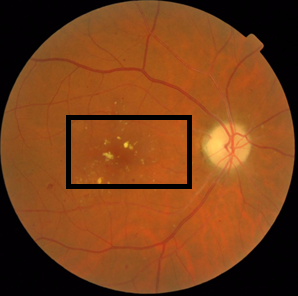
\includegraphics[width=70mm]{./Figures/cap2/microEx.png}}
\subfigure[Exudados duros.]{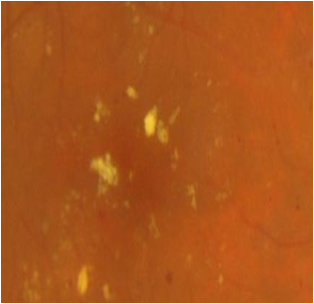
\includegraphics[width=70mm, height=70mm]{./Figures/cap2/microexu.png}}
\caption{Exudados duros.} \label{fig:sanosvsexu}
\end{figure}

\subsection{Vasos sanguíneos}
Son estructuras huecas y tubulares que conducen la sangre por el ojo. La diabetes daña estos vasos encargados de irrigar la retina. 
%El daño de los vasos sanguíneos de la retina puede tener como resultado que estos sufran una fuga de fluido o sangre. 
Cuando la enfermedad avanza se produce la creación de nuevos vasos sanguíneos  y prolifera el tejido fibroso en la retina. En la FIGURA \ref{fig:vasosgraf} se puede apreciar los vasos sanguíneos en las distintas etapas de la retinopatía diabética.

\begin{figure}[H]
\centering
\subfigure[Imagen de Retina.]{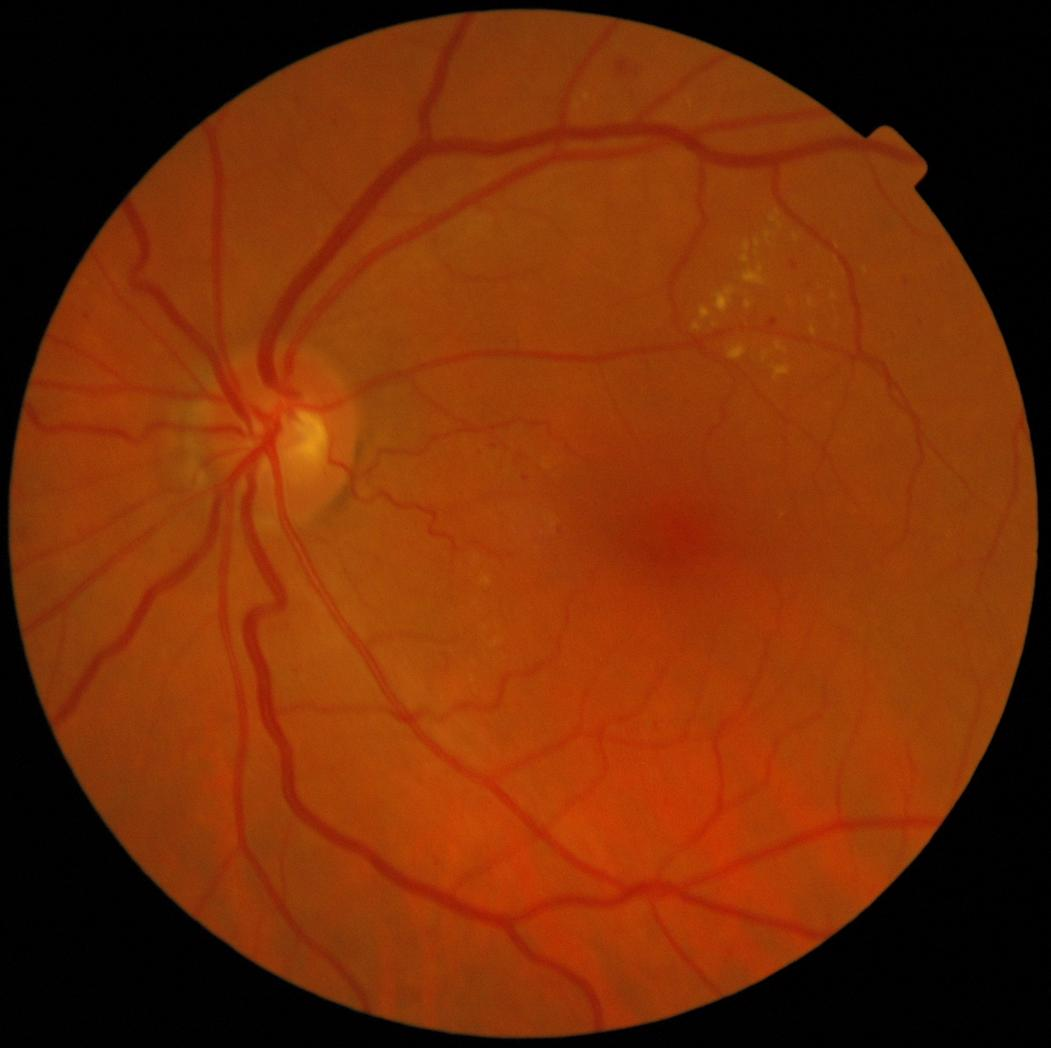
\includegraphics[width=70mm]{./Figures/cap4/vasos/vaso1.jpg}}
\subfigure[Vasos sanguíneos.]{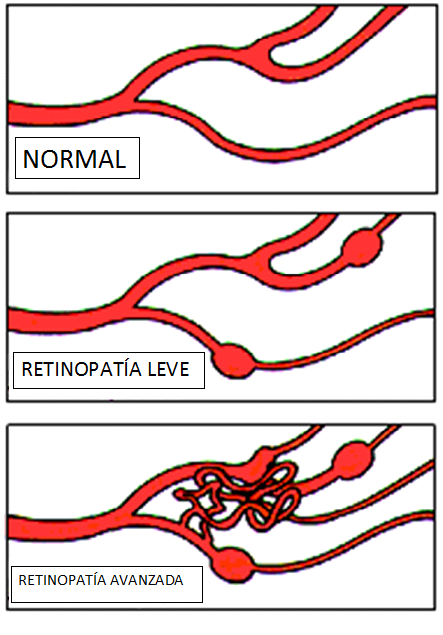
\includegraphics[width=70mm, height=70mm]{./Figures/cap2/vasosRetinpatia.png}}
\caption{Vasos sanguíneos.} \label{fig:vasosgraf}
\end{figure}

%\section{Métodos de detección}
%La detección temprana de DR es importante, porque los métodos de tratamiento pueden retrasar la progresión de la enfermedad. La mayoría de los métodos de tratamiento se basan en la tecnología láser \cite{faust2012algorithms}.

%La fotocoagulación con láser cauteriza los vasos sanguíneos oculares, que detiene con eficacia su fuga. El método de tratamiento láser focal reduce el engrosamiento de la retina. Esto puede prevenir el empeoramiento de la inflamación de la retina. Para ser más específicos, este tratamiento reduce el riesgo de pérdida de visión en un 50\% \cite{shahidi1994retinal}.


%El Análisis de imagen médica es un área de investigación que en la actualidad atrae científicos y médicos. 
%El objetivo es el desarrollo de herramientas computacionales que ayuden a la cuantificación y visualización de patologías y estructuras anatómicas. Estas herramientas funcionan con imágenes digitales de fondo de ojo. El procedimiento de la toma de imágenes de fondo de ojo se inicia mediante la dilatación de la pupila con gotas farmacéuticas para los ojos . Luego se pide al paceinte que mire a un dispositivo de fijación con el fin de estabilizar los ojos. Durante la toma las imágenes, el paciente verá una serie de destellos brillantes. Todo el proceso dura entre cinco y diez minutos. 
%Para asegurarse de que el tratamiento de DR se recibe a tiempo, las imágenes de fondo de ojo de pacientes diabéticos deben examinarse al menos una vez al año \cite{fongaiello2002diabetic}


%\subsection{Vasos sanguíneos}
%Las imágenes digitales de fondo de ojo permiten ver con claridad los vasos sanguíneos en la retina. Este método proporciona una excelente ventana para la salud de un paciente afectado por el DR. La FIGURA 3 muestra un ejemplo de detección de los vasos sanguíneos de diferentes tipos de DR [4]. La estructura de los vasos sanguíneos se obtiene sometiendo el componente verde de la imagen de fondo de ojo RGB a un número de algoritmos de procesamiento de imágenes [4].


%En \cite{chaudhuri1989detection} los vasos sanguíneos se detectaron usando filtros adaptados de dos dimensiones. El perfil de nivel de gris de la sección transversal del 
%vaso sanguíneo fue aproximado por la curva de forma gaussiana. El concepto de detección de señales de filtro adaptado se usó para detectar segmentos lineales de los vasos sanguíneos.

%Hayashe et al. ha desarrolado un sistema de diagnóstico asistido por computadora para asistir a los médicos en la detección de anormalidades asocidadas a las imágenes de fondo de retinas \cite{hayashi2001development}. Su sistema propuesto puede detectar intersecciones de vasos sanguíneos y anormalidades en el grosor de los vasos
\section{Resumen}

Como se ha comentado en este capítulo, las personas con retinopatía diabética necesariamente deben padecer diabetes, es por eso que se menciona sobre los tipos de diabetes, haciendo énfasis en que los de tipo I son más propensos a desarrollar la enfermedad. Con respecto a las estimaciones estadísticas sobre la diabetes en nuestro país, predicen un aumento de la prevalencia de personas con diabetes y que la misma avanza de manera acelerada, por lo que es de vital importancia que se pueda cubrir esta demanda de pacientes con diabetes. Es importante conocer las causas y los factores de riesgos de la retinopatía diabética de manera a tomar las precauciones pertinentes, destacando  el hecho de que recién en el estado más avanzado de la enfermedad las personas detectan los síntomas, por lo que es vital que los pacientes con diabetes se hagan el examen de fondo de ojo regularmente de tal manera a que se pueda detectar la retinopatía de forma temprana y el tratamiento pueda ser  eficaz.
Básicamente la detección de esta enfermedad radica en la exploración del fondo de ojo en busca de patologías como exudados duros y microaneurismas y así también irregularidades en las estructuras anatómicas del ojo como la neovascularización. Es esencial conocer las propiedades de coloración, formas y distribución de estas patologías y estructuras anatómicas de tal manera que se logre la implementación automática de estos y así poder asistir en el diagnóstico de esta enfermedad.
En el siguiente capítulo se presenta el marco teórico  de las técnicas de visión por computadora que se utilizan en los diferentes módulos de la metodología propuesta.



